\documentclass{article}
\usepackage[utf8]{inputenc}
\usepackage{indentfirst}
\usepackage{hyperref}
\hypersetup{
    colorlinks,
    citecolor=black,
    filecolor=black,
    linkcolor=red,
    urlcolor=blue,
}
\usepackage{graphicx}

\title{Project Management}
\author{Cinquanta Octave \\ 806286 \\ rodolphe.cinquanta@student.reutlingen-university.de}
\date{July 2022}

\begin{document}

\begin{titlepage}
    \begin{center}
        \vspace*{1cm}
            
        \Huge
        \textbf{Project Management}
            
        \vspace{0.5cm}
        \LARGE
        Magical Webshop
            
        \vspace{1.5cm}
            
        \textbf{Cinquanta Octave}
            
        \vfill
            
        \vspace{0.8cm}
            
        \Large
        Number 806286
        \vspace{0.8cm}
        rodolphe.cinquanta@student.reutlingen-university.de
        July 2022
            
    \end{center}
\end{titlepage}

\tableofcontents

\newpage
\section{Context}

This work consists in a thorough description of a startup's webshop project that aims in providing wizards around the globe with various magical ingredients, through the eyes of its manager. The goal of this work is for its writer to learn the key knowledge of Project Management, and be able to transcribe it in this work.

\section{Project Introduction}
\subsection{Overview}

Our startup's project consists in the creation of a website dedicated to selling magical ingredients to our customers. This website should provide a clear overview of all the available articles for the customers to purchase, and allow them to do so effortlessly. The website should accept and be able to handle most forms of online payment, and should also provide options for the delivery of the products to the clients. 

\subsection{Justification}

Our project exists to respond to a dire need of our customers, the need to easily find ingredients for their elixir making. Such a task often requires one to travel to several shops looking for a specific item, when a daunting task like this can be reduced to an effortless online transaction. This website will become a near necessary step in potion making due to its future usefulness and uniqueness.

\section{Work Breakdown Structure}

\begin{figure}[ht]
    \centering
    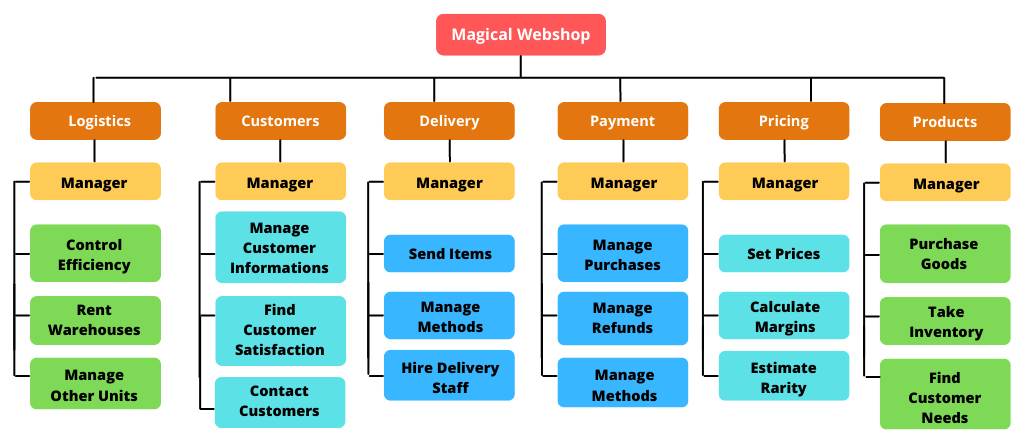
\includegraphics[width=\textwidth]{WBS.png}
    \caption{Work Breakdown Structure}
    \label{wbs}
\end{figure}

\section{Work Packages}

We shall now proceed with a description of the different work packages of our project, including their objectives, responsibilities and relationships amongst each others.

\subsection{Logistics and Warehousing}

The Logistics and Warehousing Unit is the most important unit of the project, holding the responsibility of the project's smooth operating. Its main objective is to verify and control the efficiency of the flow of goods and information throughout the project. As such this unit has the ability and duty of observing the other units' work and assessing it. Depending on this assessment, the other units' functions and structures may be influenced. This unit communicates and interacts the most with the others. It is also responsible for finding and renting suitable warehouses for the storage of the webshop's various products. Due to this duty, this unit communicates profusely with the Products Unit for the management of the company's goods.

\subsection{Customers}

The Customers Unit is the one responsible for most actions regarding our clients. Those actions include the management of their personal information, such as their names or date of birth. This sensitive data must be well managed and safely stored. Other data, including the customers' purchase histories, should be used to understand the clients' purchasing patterns and better recommend them useful items. This unit is also responsible for finding the customer's satisfaction towards our webshop. For this goal, the unit must create and implement survey tools to obtain this information, and communicate it with the rest of the project team for improvements. Lastly, this unit is in charge of communication with the customers, such as answering their inquiries and updating them on their delivery statuses. Several other units may work with the Customers Unit in the case that they need to communicate with the clients.

\subsection{Delivery}

The Delivery Unit is responsible for the work surrounding the delivery system. That includes the deliveries themselves : from packaging the items to sending them out to the clients, and overseeing everything in between. This unit must also manage the various delivery methods. This means implementing different methods based on the needs of the customers, the realism of the implementation and its costs, ideally creating a range of delivery methods adapted to the customers' budgets and situations. The Customers Unit will provide this unit the necessary information. Finally, this unit is also responsible for hiring the delivery staff and managing it. The staff will be formed and sent to the field as the unit sees fit.

\subsection{Payment}

The Payment Unit is responsible for dealing with the monetary transactions between the company and the customers. That includes managing the client's purchases and providing them with the ability to obtain refunds. This unit will be the link between financial institutions such as banks and neutral third parties providing money transfer services. This unit shall treat the client's financial data carefully and ensure the correctness of the transactions. This unit should also manage the different payment methods, and aim to implement as many of them as realistically possible. By multiplying the payment methods, the number of clients making purchases will increase, and such is a major responsibility of this unit.

\subsection{Pricing}

The Pricing Unit is responsible for the management of the monetary value of the company's products. This unit has a duty of assigning a price to each merchantable product, and that price must be inferred using several important criteria. Those criteria are linked to this unit's other two responsibilities. The first one is the calculate the margins the company needs to impose on the prices in order to keep a sustainable economy and guarantee positive profits. Those margins should be increased or decreased depending on the difficulty or ease of access to a raw product. The second is to estimate the rarity of the products. This unit needs to comprehend the nature of the product's origins and usual whereabouts in order to consider its complete value and adjust its price accordingly. The realisation of those two tasks allows for a correct setting of the prices.

\subsection{Products}

The Products Unit is responsible for the management of the company's products in cooperation with the Logistics and Warehousing Unit. Whereas the first unit manages the storage of the goods, this unit is tasked with purchasing the goods. This includes the necessary research and communication with various suppliers around the world. Contracts involving buying products in large quantities at once are to be obtained if possible. This unit is also responsible for taking the inventory, keeping track of the available and stock amount of each product whenever one is sold or bought. When the company is starting to lack a certain item, this unit is responsible for noticing this issue and resolving it. At last, this unit has also as duty to research what items are currently the most requested or needed by the customers and organise their purchase. Such a research is not this unit's major task, however it stays important and should be done regularly. This unit may need the cooperation of the Customers Unit for its research.

\section{Milestone Plan}

\begin{figure}[ht]
    \centering
    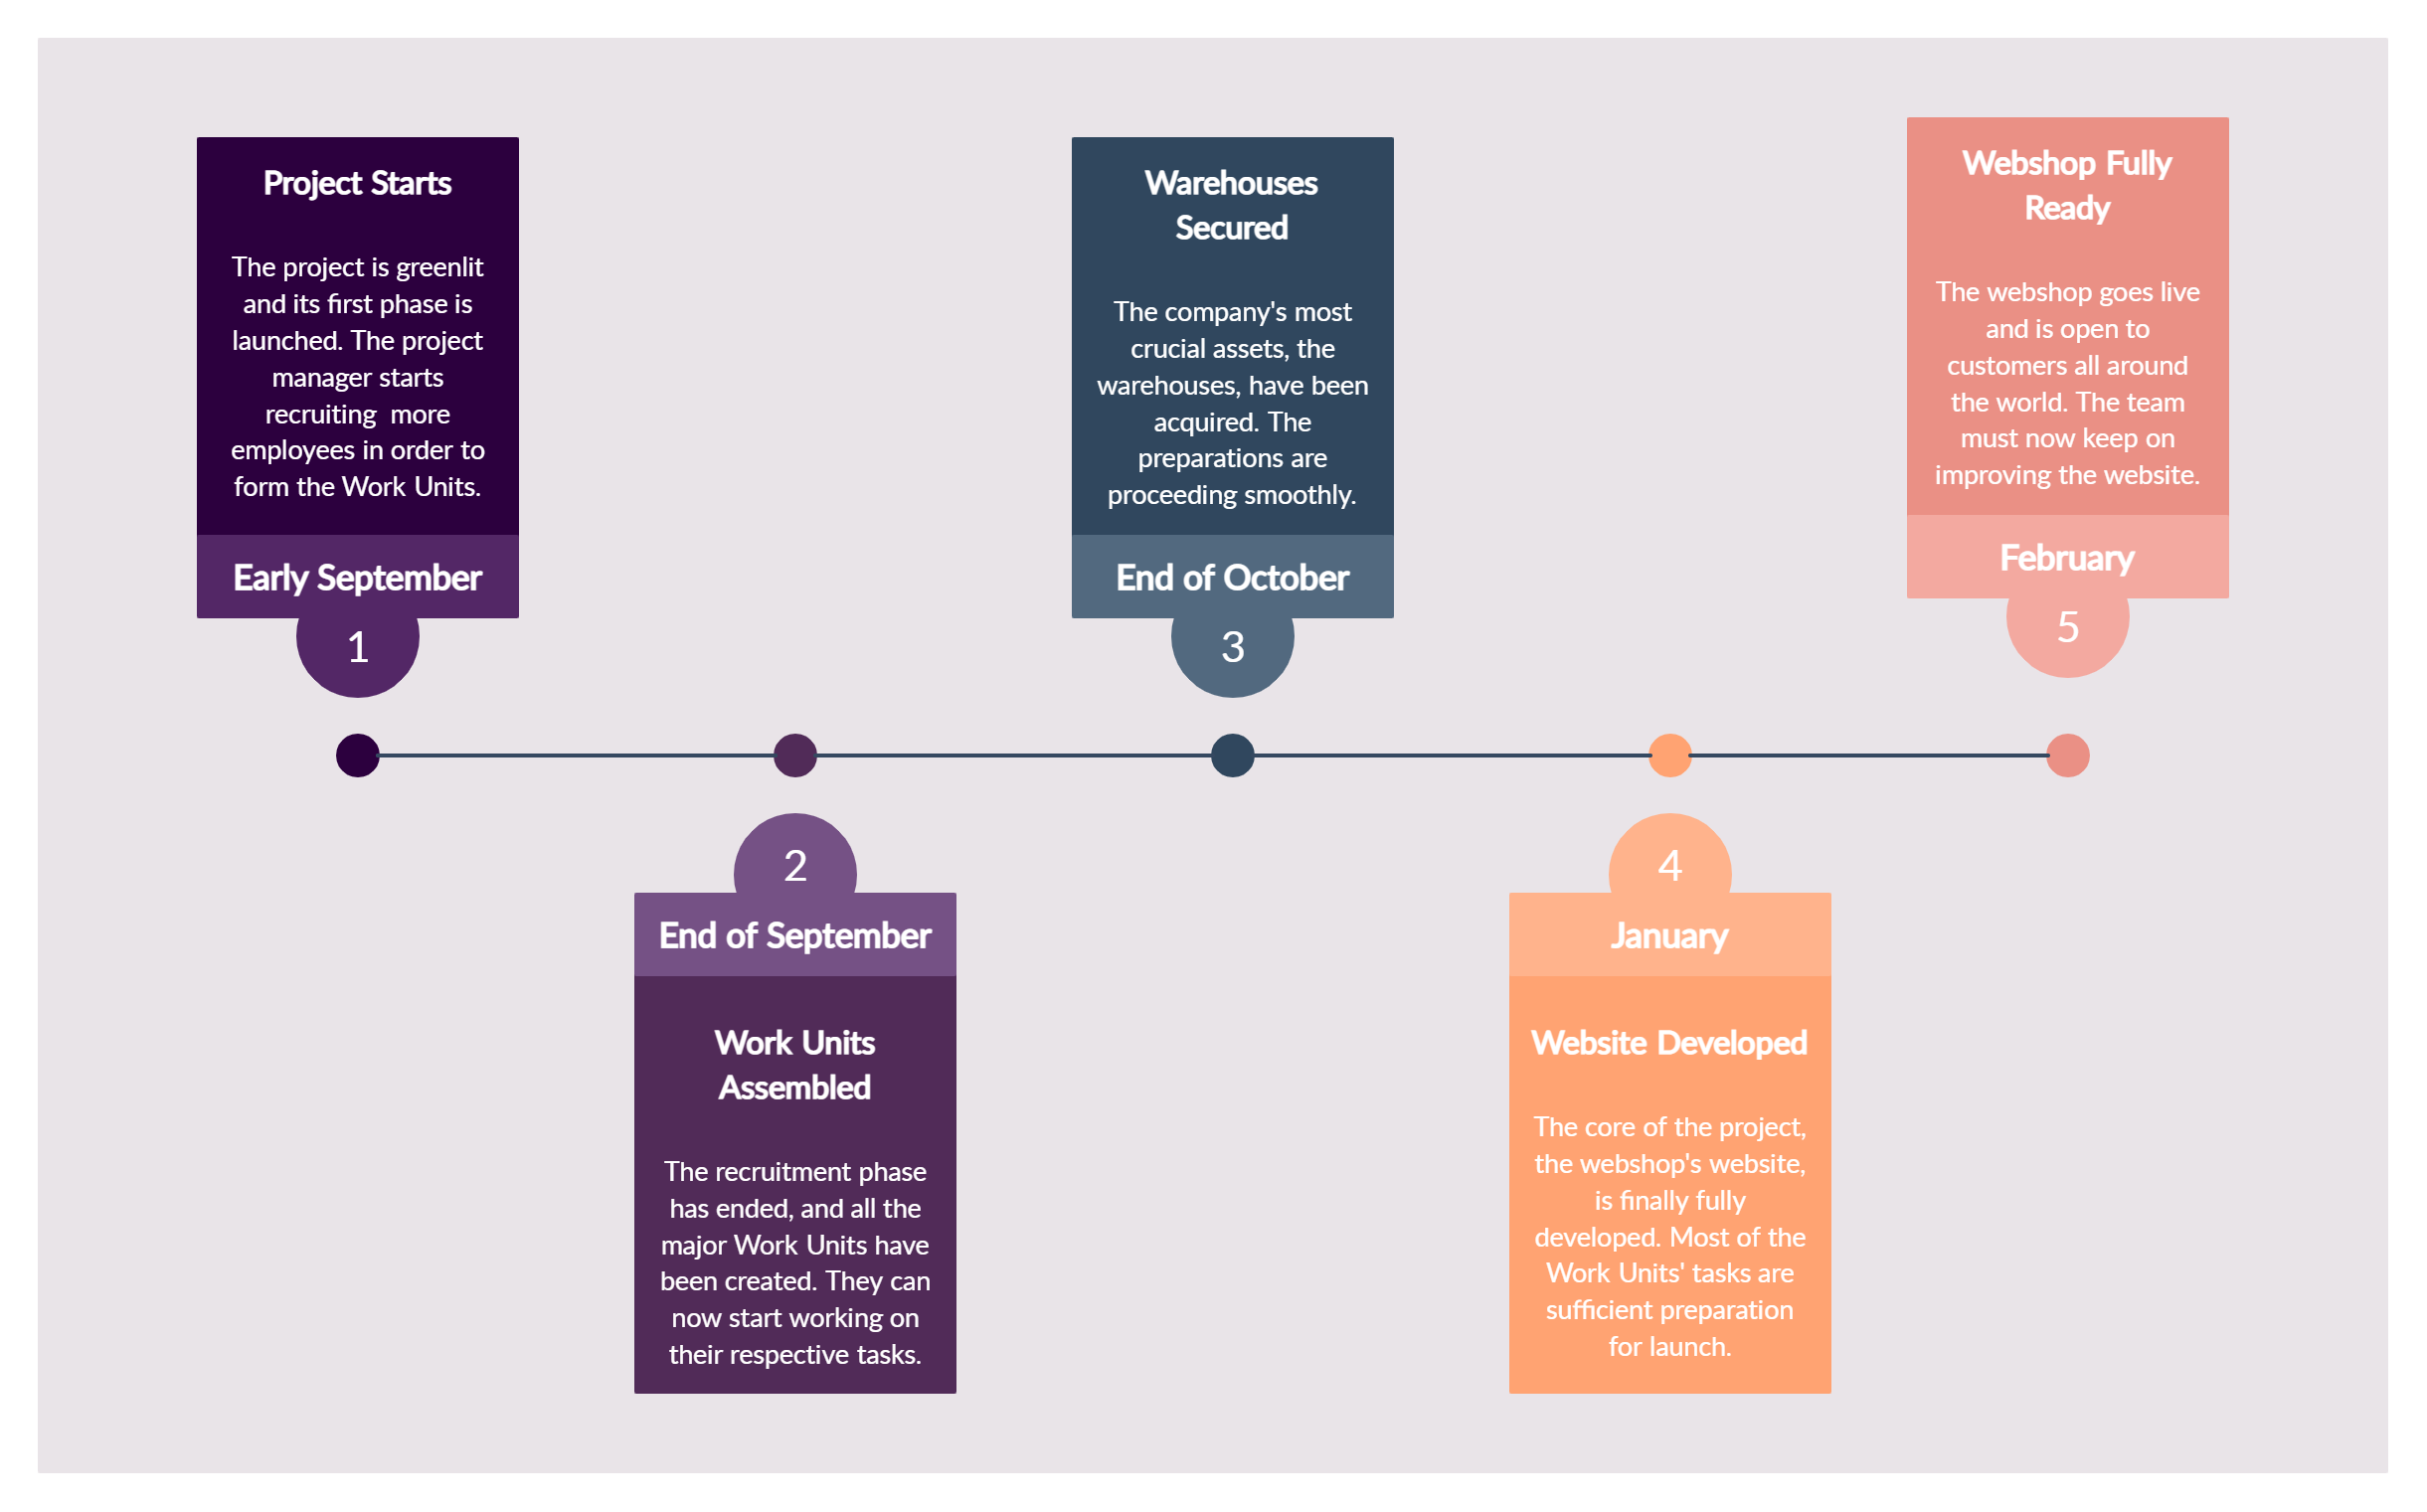
\includegraphics[width=\textwidth]{Milestone Plan.png}
    \caption{Milestone Plan}
    \label{plan}
\end{figure}

\section{Reference List}

\begin{itemize}
    \item Project Management Institute (2021), \textit{A Guide to the Project Management Body of Knowledge}
    \item Greg Horine (2005), \textit{Project Management: Absolute Beginner’s Guide}
\end{itemize}

\end{document}
